\section{证明}
\subsection{\ref{eq:hyperbolic_functions_1}}
\begin{displaymath}
\begin{split}
\sinh x\cosh x &= \left(\frac{e^x-e^{-x}}{2}\right)\left(\frac{e^x+e^{-x}}{2}\right) \\
&=\left(\frac{1}{2}\right)\left(\frac{e^{2x}-e^{-2x}}{2}\right) \\
&= \frac{1}{2}\sinh (2x) \\
\sinh (2x) &= 2\sinh x\cosh x
\end{split}
\end{displaymath}

\subsection{\ref{eq:hyperbolic_functions_2}}
\begin{displaymath}
\begin{split}
\cosh^2x-\sinh^2x &=\left(\frac{e^x+e^{-x}}{2}+\frac{e^x-e^{-x}}{2}\right)\left(\frac{e^x+e^{-x}}{2}-\frac{e^x-e^{-x}}{2}\right) \\
&= e^x\times e^{-x} \\
&=1
\end{split}
\end{displaymath}

\subsection{\ref{eq:hyperbolic_functions_3}}
\begin{displaymath}
\begin{split}
\cosh^2x+\sinh^2x &=\left(\frac{e^x+e^{-x}}{2}\right)^2+\left(\frac{e^x-e^{-x}}{2}\right)^2 \\
&=\frac{2e^{2x}+2e^{-2x}}{4} \\
&=\frac{e^{2x}+e^{-2x}}{2} \\
&=\cosh (2x)
\end{split}
\end{displaymath}

\subsection{\ref{eq:hyperbolic_functions_4}}
\begin{displaymath}
\begin{split}
\cosh (2x)  &=\cosh^2x+\sinh^2x \\
&=\sinh^2x +1 +\sinh^2x \\
&=2\sinh^2x +1 \\
\cosh x &=2\sinh^2\frac{x}{2}+1
\end{split}
\end{displaymath}
\subsection{\ref{sequence_bounded_1}}
    \begin{center}
       $\varepsilon =1,\ \exists N>0,\ \mbox{当n>N时}\left|X_n-a\right|<1$\\
        $\left|X_n\right|=\left|(X_n-a)+a\right|$\\
        $\qquad\leqslant \left|x_n-a\right|+\left|a\right|$\\
        $\leqslant 1+\left|a\right|$\\
        $M=\max\{\left|X_n\right|,\left|X_2\right|,\dots,\left|X_n\right|,1+\left|a\right|\}$\\
        $\forall n,\ \left|X_n\right|\leqslant M$
    \end{center}
\subsection{\ref{Serial_number_preservation_a}}
    \begin{center}1\end{center}
    $\mbox{由于}\lim\limits_{n\to\infty}x_n = a,\mbox{且}a>0$\\
    $\varepsilon = \frac{a}{2},\ \exists N>0,n>N$\\
    $\left|x_n-a\right|<\varepsilon$\\
    $\left|x_n-a\right|<\frac{a}{2}$\\
    $-\frac{a}{2}<x_n-a<\frac{a}{2}$\\
    $\frac{a}{2}<x_n<1$
    \begin{center}2\end{center}
    用反证法,反设$a<0$.从某项起$x_n<0$矛盾
\subsection{\ref{Serial_number_preservation_b}}
\begin{displaymath}
    \begin{split}
        x_n&=b_n-a_n\\
        \lim\limits_{n\to\infty} x_n &= \lim\limits_{n\to\infty} b_n-\lim\limits_{n\to\infty}a_n\\
        \lim\limits_{n\to\infty} x_n &=b-a>0\\
        \lim\limits_{n\to\infty} x_n &>0 \\
        b_n-a_n&=x_n > 0\\
        b_n&>a_n
    \end{split}
\end{displaymath}

\subsection{\ref{limit_sequence}}
\begin{displaymath}
    \begin{split}
        \mbox{反设}&\lim\limits_{n \to \infty}x_n =a,\ \lim\limits_{n \to \infty}x_n =b,\mbox{且}a<b\\
        \varepsilon&=\frac{b-a}{3}\begin{cases}
            \exists N_1,\ n>N_1,\ \left|x_n-a\right|<\frac{b-a}{3}\\
            \exists N_2,\ n>N_2,\ \left|x_n-b\right|<\frac{b-a}{3}
        \end{cases}\\
        N&=\max\{N_1,N_2\},\ n>N\Rightarrow\begin{cases}
            n>N_1\\
            n>N_2
        \end{cases}\\
        b-a&=\left|(x_n-a)-(x_n-b)\right|\\
        &\leqslant \left|x_n-a\right|+\left|x_n-b\right|\\
        &<\frac{b-a}{3}+\frac{b-a}{3}\\
        &<\frac{2(b-a)}{3}
    \end{split}
\end{displaymath}
\subsection{\ref{limit_left_right}}
$\lim\limits_{x\to x_0}f(x)\mbox{存在}\Rightarrow \lim\limits_{x\to x_0^+}f(x)=\lim\limits_{x\to x_0^-}f(x)$
\begin{center}
    设$\lim\limits_{x\to x_0}=A$\\
    $0<\left|x-x_0\right|<\delta,\ \left|f(x)-A\right|<\varepsilon$\\
    $0<\left|x-x_0\right|<\delta\Leftrightarrow x\in \mathring{U}(x_0,\delta)$
    $\begin{cases}
        \mbox{当}x_0<x<x_0+\delta\mbox{时}0<\left|x-x_0\right|<\delta,\ \left|f(x)-A\right|<\varepsilon,\ \lim\limits_{x\to x_0^+}f(x)=A\\
        \mbox{当}x_0-\delta<x<x_0\mbox{时}0<\left|x-x_0\right|<\delta,\ \left|f(x)-A\right|<\varepsilon,\ \lim\limits_{x\to x_0^-}f(x)=A
    \end{cases}$
    $\lim\limits_{x\to x_0^+}f(x)=A =\lim\limits_{x\to x_0^-}f(x)$
\end{center}
$\lim\limits_{x\to x_0}f(x)\mbox{存在}\Leftarrow\lim\limits_{x\to x_0^+}f(x)=\lim\limits_{x\to x_0^-}f(x)$
\begin{center}
    $A=\begin{cases}
    \lim\limits_{x\to x_o^+},\forall\varepsilon>0,\exists\delta_1>0,x_0<x<x_0+\delta_1,\left|f(x)-A\right|<\varepsilon\\
    \lim\limits_{x\to x_o^-},\forall\varepsilon>0,\exists\delta_2>0,x_0-\delta_2<x<x_0,\left|f(x)-A\right|<\varepsilon\\
    \end{cases}$\\
    $\delta = \min\{\delta_1,\delta_2\}$\\
    $0<\left|x-x_0\right|<\delta\begin{cases}
        x>x_0,x_0<x<x_0+\delta\leqslant x_0+\delta_1,\  \left|f(x)-A\right|<\varepsilon\\
        x<x_0,x_0-\delta_2\leqslant x_0+\delta<x<x_0,\ \left|f(x)-A\right|<\varepsilon
    \end{cases}$\\
    $\lim\limits_{x\to x_0}f(x)=A$
\end{center}
\subsection{\ref{limit_infinitesimal}}
$$\lim\limits_{x\to x_o}f(x)=A\Rightarrow \begin{cases}
    \alpha\mbox{为}x\rightarrow x_0 \mbox{时的无穷小}\\
    f(x)=\alpha+A
\end{cases}$$
设$\lim\limits_{x\to x_o}f(x)=A,\ \mbox{记}f(x)-A=\alpha$\\
只需证$\alpha$为无穷小。\\
$\forall\varepsilon>0,\exists\delta>0,\mbox{当}0<\left|x-x_0\right|<\delta,\mbox{时}\left|f(x)-A\right|<\varepsilon$\\
即$\left|\alpha-0\right|<\varepsilon$\\
$\alpha\mbox{为}x\rightarrow x_0\mbox{时的无穷小}$
$$\lim\limits_{x\to x_o}f(x)=A\Leftarrow \begin{cases}
    \alpha\mbox{为}x\rightarrow x_0 \mbox{时的无穷小}\\
    f(x)=\alpha+A
\end{cases}$$
$\forall \varepsilon >0,\ \exists \delta >0,\ \mbox{当}0<\left|x-x+0\right|<\delta,\ \left|\alpha\right|<\varepsilon$\\
$\mbox{即}\left|f(x)-A\right|<\varepsilon$
$\lim\limits_{x\to x_0}f(x)=A$
\subsection{\ref{Infinity_infinitesimal}}
\begin{center}
    设$\lim\limits_{x\to x_0}f(x)=\infty$\\
对$f(x)$为$x\rightarrow$时无穷大\\
对于$M=\frac{1}{\varepsilon}$.存在$\delta>0$\\
当$0<\left|x-x_0\right|<\delta$时\\
$\left|f(x)\right|>M=\frac{1}{\varepsilon}$\\
$\left|\frac{1}{f(x)}\right|<\varepsilon$\\
$\frac{1}{f(x)}$为$x\rightarrow x_0$时的无穷小
\end{center}
\subsection{\ref{Extreme Four Operations_2}}
\begin{displaymath}
    \begin{split}
        f(x)g(x)&=\left[A+\alpha\right]\left[B+\beta\right]\\
        &=AB+A\beta+B\alpha+\beta\alpha\\
        &=AB+\gamma\qquad\qquad(\gamma\mbox{为无穷小})\\
        \lim\left[f(x)g(x)\right]&=AB+\gamma=\lim f(x)\lim g(x)
    \end{split}
\end{displaymath}

\subsection{\ref{eq:squeeze_theorem}}
\begin{center}
    $\forall \varepsilon > 0$\\
$\left|x_n-a\right|<\varepsilon\qquad\forall n>N_1$\\
$\left|y_n-a\right|<\varepsilon\qquad\forall n>N_2$\\
$\mbox{令}N = \max\left\{{N_1,N_2,N_0}\right\}\mbox{,则当}n > N\mbox{时有}$\\
$a-\varepsilon<x_n\le z_n\le y_n < a+\varepsilon$\\
$\left|z_n-a\right|<\varepsilon$\\
$\lim\limits_{{n}\to{\infty}}z_n = a$
\end{center}

\subsection{\ref{limit_1_1}}
\begin{center}
    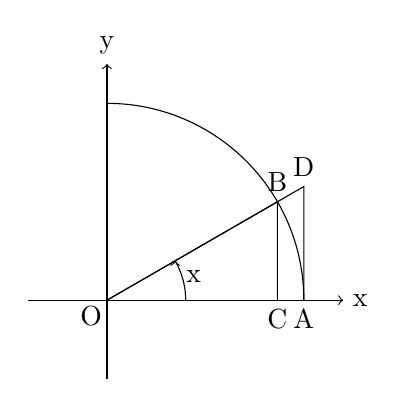
\begin{tikzpicture}[>=to]
        \begin{scope}
            \draw[->] (-1,0)--(3,0)node[right]{x};
            \draw[->] (0,-1)--(0,3)node[above]{y};
            \draw[] (2.5,0) arc(0:90:2.5) (1,2.5);
            \draw[->] (1,0) arc(0:30:1) ({cos (pi/6 r)},{sin (pi/6 r)});
            \draw (0,0)--(30:2.5)node[above]{B}--({(2.5)*(cos (pi/6 r))},0)node[below]{C};
            \draw (0,0)--(2.5,{(2.5)*(tan (pi/6 r))})node[above]{D}--(2.5,0)node[below]{A};
            \node at (-.2,-.2) {O};
            \node at (1.1,.3) {x};
        \end{scope}
    \end{tikzpicture}\\
    \begin{displaymath}
        \begin{split}
            OB&=OA=1\\
            \vartriangle AOB&\leqslant \mbox{扇形面积}\leqslant\vartriangle AOD\\
            \frac{1}{2}\sin x&\leqslant\frac{1}{2}x\leqslant\frac{1}{2}\tan x\\
            \sin x&\leqslant x\leqslant \tan \\
            1&\geqslant\frac{\sin x}{x}\geqslant \cos x\\
            \lim\limits_{x\to 0}1&\geqslant\lim\limits_{x\to 0}\frac{\sin x}{x}\geqslant\lim\limits_{x\to 0}\cos x\\
            1&\geqslant\lim\limits_{x\to 0}\frac{\sin x}{x}\geqslant1\\
            \lim\limits_{x\to 0}\frac{\sin x}{x} &= 1
        \end{split}
    \end{displaymath}
\end{center}
\subsection{\ref{limit_1_2}}
\begin{displaymath}
    \centering
    \begin{split}
        \left|1-\cos x\right|=1-\cos x&=2\sin^2 \frac{x}{2}\\
        &\leqslant 2\left(\frac{x}{2}\right)^2\\
        0\leqslant 1-\cos x &\leqslant \frac{x^2}{2}\\
        \lim\limits_{x\to 0}0\leqslant\lim\limits_{x\to 0}\left(1-\cos x\right)&\leqslant\lim\limits_{x\to 0}{\frac{x^2}{2}}\\
        0\leqslant\lim\limits_{x\to 0}\left(1-\cos x\right)&\leqslant 0\\
        \lim\limits_{x\to 0}\left(1-\cos x\right) &=0\\
        \lim\limits_{x\to 0}\cos x&=1
    \end{split}
\end{displaymath}
\subsection{\ref{limit_1_3}}
\begin{displaymath}
    \centering
    \begin{split}
        \lim\limits_{x\to 0}\frac{\tan x}{x}&=\lim\limits_{x\to 0}\frac{\sin x}{x}\frac{1}{\cos x}\\
        &=\lim\limits_{x\to 0}\frac{\sin x}{x}\lim\limits_{x\to 0}\frac{1}{\cos x}\\
        &=1
    \end{split}
\end{displaymath}
\subsection{\ref{limit_1_4}}
\begin{displaymath}
    \centering
    \begin{split}
        \lim\limits_{x\to 0}\frac{1-\cos x}{\frac{1}{2}x^2}&=\lim\limits_{x\to 0}\frac{2\sin^2\frac{x}{2}}{\frac{1}{2}x^2}\\
        &=\lim\limits_{x\to 0}\left(\frac{\sin \frac{x}{2}}{\frac{x}{2}}\right)^2\\
        &=1
    \end{split}
\end{displaymath}
\subsection{\ref{limit_1_5}}
\begin{displaymath}
    \centering
    \begin{split}
        x=\sin t,\ t=\arcsin x\\ 
        x\rightarrow 0,\ t\rightarrow 0\\
        \lim\limits_{x\to 0}\frac{\arcsin x}{x}=\lim\limits_{x\to 0}\frac{t}{\sin t}=1
    \end{split}
\end{displaymath}
\subsection{\ref{limit_1_6}}
\begin{displaymath}
    \centering
    \begin{split}
        x=\tan t,\ t=\arctan x\\ 
        x\rightarrow 0,\ t\rightarrow 0\\
        \lim\limits_{x\to 0}\frac{\arctan x}{x}=\lim\limits_{t\to 0}\frac{t}{\tan t}=1
    \end{split}
\end{displaymath}
\subsection{\ref{limit_1_7}}
\begin{displaymath}
    \centering
    \begin{split}
        \lim\limits_{x\to 0}\frac{\ln \left(1+x\right)}{x}=\lim\limits_{x\to 0}\ln \left(1+x\right)^\frac{1}{x}=\ln e=1
    \end{split}
\end{displaymath}
\subsection{\ref{limit_1_8}}
\begin{displaymath}
    \centering
    \begin{split}
        e^x-1=t,\ x=\ln\left(t+1\right)\\
        x\rightarrow 0,\ t\rightarrow 0\\
        \lim\limits_{x\to 0}\frac{e^x-1}{x}=\lim\limits_{t\to 0}\frac{t}{\ln\left(t+1\right)}=1
    \end{split}
\end{displaymath}
\subsection{\ref{limit_1_9}}
\begin{displaymath}
    \centering
    \begin{split}
        \lim\limits_{x\to 0}\frac{\left(1+x\right)^n-1}{nx}=\lim\limits_{x\to 0}\left(\frac{e^{n\ln \left(1+x\right)}-1}{n\ln\left(1+x\right)}\cdot\frac{\ln\left(1+x\right)}{x}\right)=1
    \end{split}
\end{displaymath}

\subsection{\ref{limit_2_1}}
\begin{displaymath}
    \centering
    \begin{split}
        x_n&=\left(1+\frac{1}{n}\right)^n=\sum_{m = 0}^{n} C_n^m 1^{n-m}\left(\frac{1}{n}\right)^m=\sum_{m = 0}^{n} C_n^m \left(\frac{1}{n}\right)^m\\
        &=C_n^0\left(\frac{1}{n}\right)^0+C_n^1\left(\frac{1}{n}\right)^1+ \sum_{m = 2}^{n} C_n^m \left(\frac{1}{n}\right)^m\\
        &=1+1+ \sum_{m = 2}^{n} \frac{n!}{m!\left(n-m\right)!} \left(\frac{1}{n}\right)^m\\
        &=1+1+ \sum_{m = 2}^{n} \frac{\overbrace{\left(n\right)\left(n-1\right)\cdots\left(n-m+1\right)}^{m}}{m!} \left(\frac{1}{n}\right)^m\\
        &=1+1+ \sum_{m = 2}^{n} \frac{1}{m!}\left(\frac{n}{n}\right)\left(\frac{n-1}{n}\right)\cdots\left(\frac{n-m+1}{n}\right) \\
        &=1+1+ \sum_{m = 2}^{n} \frac{1}{m!}\left(1-\frac{1}{n}\right)\left(1-\frac{2}{n}\right)\cdots\left(1-\frac{m-1}{n}\right) \\
        x_{n+1}&=1+1+ \sum_{m = 2}^{n+1} \frac{1}{m!}\left(1-\frac{1}{n+1}\right)\left(1-\frac{2}{n+1}\right)\cdots\left(1-\frac{m-1}{n+1}\right) \\
        x_n&<x_{n+1}\qquad\mbox{单调增加}\\
        x_n&<1+1+\frac{1}{2!}+\frac{1}{3!}+\cdots+\frac{1}{n!}\\
        &<1+1+\frac{1}{2^2}+\frac{1}{2^3}+\cdots+\frac{1}{n^2}=1+\frac{1-\left(\frac{1}{2}\right)^2}{1-\frac{1}{2}}\\
        &<1+\frac{1}{1-\frac{1}{2}}\\
        &<3\qquad \mbox{有界}
    \end{split}
\end{displaymath}

\subsection{\ref{derivative_1}}
\begin{displaymath}
    \centering
    \begin{split}
        \frac{d}{\mathrm{d}{x}}C&=\lim\limits_{\vartriangle x\to 0}\frac{f(x_0+\vartriangle x)-f(x_0)}{\vartriangle x}\\
        &=\lim\limits_{\vartriangle x\to 0} \frac{C-C}{\vartriangle x}\\
        &=0
    \end{split}
\end{displaymath}

\subsection{\ref{derivative_2}}
\begin{displaymath}
    \centering
    \begin{split}
        \frac{d}{\mathrm{d}{x}}x^a&=\lim\limits_{x\to x_0}\frac{f(x)-f(x_0)}{x-x_0}\\
        &=\frac{x^a-x_0^a}{x-x_0}\\
        &=\frac{(x-x_0)\left(x^{a-1}+x^{a-2}x_0+\cdots+xx_0^{a-2}+x_0^{a-1}\right)}{x-x_0}\\
        &=ax_0^{a-1}
    \end{split}
\end{displaymath}

\subsection{\ref{derivative_3}}
\begin{displaymath}
    \centering
    \begin{split}
        \frac{d}{\mathrm{d}{x}}a^x&=\lim\limits_{\vartriangle x\to 0}\frac{a^{x+\vartriangle x}-a^x}{\vartriangle x}\\
        &=a^x\lim\limits_{\vartriangle x\to 0}\frac{a^{\vartriangle x}-1}{\vartriangle x}\\
        &=a^x\lim\limits_{\vartriangle x\to 0}\frac{e^{\vartriangle x \ln a}-1}{\vartriangle x}\\
        &=a^x\ln a
    \end{split}
\end{displaymath}

\subsection{\ref{derivative_4}}
\begin{displaymath}
    \begin{split}
        \frac{d}{\mathrm{d}{x}}e^x=e^x\ln e=e^x
    \end{split}
\end{displaymath}
\subsection{\ref{derivative_5}}
\begin{displaymath}
    \centering
    \begin{split}
        \frac{d}{\mathrm{d}{x}}\log_a^x&=\lim\limits_{\vartriangle x\to 0}\frac{\log_a^{x+\vartriangle x}-\log_a^x}{\vartriangle x}\\
        &=\lim\limits_{\vartriangle x\to 0}\frac{\log_a^{1+\frac{\vartriangle x}{x}}}{\vartriangle x}\\
        &=\lim\limits_{\vartriangle x\to 0}\frac{\ln{1+\frac{\vartriangle x}{x}}}{\ln a\vartriangle x}\\
        &=\frac{1}{\ln a}\lim\limits_{\vartriangle x\to 0}\frac{\frac{\vartriangle x}{x}}{\vartriangle x}\\
        &=\frac{1}{x\ln a}
    \end{split}
\end{displaymath}
\subsection{\ref{derivative_6}}
\begin{displaymath}
    \begin{split}
        \frac{d}{\mathrm{d}{x}}\ln^x&=\frac{1}{x\ln e}\\
        &=\frac{1}{x}
    \end{split}
\end{displaymath}
\subsection{\ref{derivative_sin}}
\begin{displaymath}
    \centering
    \begin{split}
        \frac{d}{\mathrm{d}{x}}\sin x&=\lim\limits_{\vartriangle x\to 0}\frac{f(x_0+\vartriangle x)-f(x_0)}{\vartriangle x}\\
        &=\frac{\sin (x_0 +\vartriangle x)-\sin x_0}{\vartriangle x}\\
        &=\frac{2\cos(x_0+\frac{\vartriangle x}{2})\sin \frac{\vartriangle x}{2}}{\vartriangle x}\\
        &=\cos(x_0+\frac{\vartriangle x}{2})\frac{\sin\frac{\vartriangle x}{2}}{\frac{\vartriangle x}{2}}\\
        &=cos x_0
    \end{split}
\end{displaymath}
\subsection{\ref{derivative_cos}}
\begin{displaymath}
    \centering
    \begin{split}
        \frac{d}{\mathrm{d}{x}}\cos x&=\lim\limits_{\vartriangle x\to 0}\frac{f(x_0+\vartriangle x)-f(x_0)}{\vartriangle x}
    \end{split}
\end{displaymath}

